%; whizzy-master "main.tex"

\chapter{Specification language}
\label{chap:base}

\section{Lexical rules}

Lexical structure mostly follows that of ANSI C. A few differences
must be noted:
\begin{itemize}
\item the character \verb|'@'| is a blank character, thus equivalent
  to a space character.
\item the identifiers may start with the backslash character.
\end{itemize}

\experimental

\begin{itemize}
\item Some UTF8 characters may be used in place of some constructs: $\leq$ for \verb|<=|, $\forall$ for \Forall, etc.
\end{itemize}

\section{Logic expressions}
\label{sec:expressions}

This first section presents the language of expressions one can use in
annotations. These are called below \emph{logic expressions}. They
correspond to pure C expressions, with additional constructs
that we will introduce progressively.

\begin{figure}[p]
  \fbox{\begin{minipage}{0.97\textwidth} \begin{syntax}
  bin-op ::= "+" | "-" | "*" | "/" | "%" ;
       | "==" | "!=" | "<=" | ">=" | ">" | "<" ;
       | "&&" | "||" |   ; boolean operations
       | "&" | "|" | {"--->"} | {"<--->"} | "^"; bitwise operations
       \
  unary-op ::= "+" | "-" ; unary plus and minus
       | "!" ; boolean negation
       | "~" ;  bitwise complementation
       | "*" ; pointer dereferencing
       | "&" ; address-of operator
       \
  term ::= "\true" | "\false" ;
       | integer ; integer constants
       | real ; real constants
       | id ; variables
       | unary-op term ;
       | term bin-op term ;
       | term "[" term "]" ; array access
       | "{" term "for" "[" term "]" "=" term "}" ; array functional modifier
       | term "." id  ; structure field access
       | "{" term "for" id "=" term "}" ; structure field functional modifier
       | term "->" id ;
       | "(" type-expr ")" term  ; cast
       | id "(" term ("," term)* ")" ; function application
       | "(" term ")" ; parentheses
       | term "?" term ":" term ;
       | {"\let" id "=" term ";" term} ; local binding
       | "sizeof" "(" term ")" ;
       | "sizeof" "(" C-type-expr ")" ;
       | id ":" term ; syntactic naming
       \
  rel-op ::= "==" | "!=" | "<=" | ">=" | ">" | "<"
       \
  pred ::= "\true" | "\false" ;
       | term (rel-op term)+ ; comparisons (see remark)
       | id "(" term ("," term)* ")" ; predicate application
       | "(" pred ")" ; parentheses
       | pred "&&" pred ; conjunction
       | pred "||" pred ; disjunction
       | pred "==>" pred ; implication
       | pred "<==>" pred ; equivalence
       | "!" pred ; negation
       | pred "^^" pred ; exclusive or
       | term "?" pred ":" pred ;
       | { pred "?" pred ":" pred };
       | { "\let" id "=" term ";" pred }; local binding
       | "\forall" binders ";" pred ; universal quantification
       | "\exists" binders ";" pred ; existential quantification
       | id ":" pred ; syntactic naming
\end{syntax}

%%% Local Variables:
%%% mode: latex
%%% TeX-master: "main"
%%% End:

    \end{minipage}}
  \caption{Grammar of terms and predicates}
\label{fig:gram:term}
\end{figure}

Figure~\ref{fig:gram:term} presents the grammar for the basic
construction of logic expressions.  In that grammar, we distinguish
between \emph{predicates} and \emph{terms}, following the usual
distinction between propositions and terms in classical first-order
logic.  The grammar for binders and type expression is given
separately in Figure~\ref{fig:gram:binders}.

With respect to C pure expressions, the additional constructs are as follows:
\begin{description}
\item[Additional connectives]
  C operators \verb|&&|, \verb+||+ and \verb|!| are used as
  logical connectives. There are additional connectives \verb|==>| for
  implication, \verb|<==>| for equivalence and \verb|^^| for exclusive
  or. These logical connectives all have a bitwise counterpart, either
  C ones like \verb|&|, \verb+|+, \verb|~| and \verb|^|, or additional
  ones like the bitwise implication \verb|-->| and the bitwise
  equivalence \verb|<-->|.

\item[Quantification] Universal quantification is denoted by $\Forall
  \tau~x_1,\ldots,x_n; e$ and existential quantification by $\Exists
  \tau~ x_1,\ldots,x_n; e$.

\begin{figure}[t]
  \fbox{\begin{minipage}{0.97\textwidth} \begin{syntax}
  binders ::= type-expr variable-ident ("," variable-ident)*
  \
  type-expr ::= logic-type-expr | C-type-expr
  \
  logic-type-expr ::= built-in-logic-type ;
  | id ; type identifier
  | "'" id ; type variable
  | type-expr id ; polymorphic type                 
  | "(" type-expr (, type-expr)* ")" id ; polymorphic type
  | logic-type-expr ("*" logic-type-expr)+  ; \experimental product type 
  \
  built-in-logic-type ::= "boolean" | "integer" | "real" 
  \
  variable-ident ::= id 
  | "*" variable-ident 
  | variable-ident "[]"
\end{syntax}
    \end{minipage}}
  \caption{Grammar of binders and type expressions}
\label{fig:gram:binders}
\end{figure}

\item[Local binding] $\Let x = e_1 ; e_2$ introduces the name $x$ for
  expression $e_1$ which can be used in expression $e_2$.

\item[Conditional] $c ? e_1 : e_2$. There is a subtlety
  here: the condition may be either a boolean term or a predicate.  In
  case of a predicate, the two branches must be also predicates, so
  that this construct acts as a connective with the following
  semantics: $ c ? e_1 : e_2$ is equivalent to $(c
  \verb|==>| e_1) \verb|&&| (\verb|!| c \verb|==>| e_2)$

\item[Syntactic naming] $id \verb|:| e$ is a term or a predicate
  equivalent to $e$. It is different from local naming with $\Let$:
  the name cannot be reused in other terms of predicates. It is only
  for readibility purposes.

\item[Logic functions] applications in terms and in propositions are not
applications of C functions, but of logic functions or predicates: see
Section~\ref{sec:logicspec} for detail.

\item[Consecutive comparison operators] the construct $t_1~relop_1~t_2~relop_2~t_3 \cdots t_k$ with
  several consecutive comparison operators is a shortcut for
  $t_1~relop_1~t_2 ~\verb|&&|~ t_2~relop_2~t_3 ~\verb|&&|~ \cdots $.
  Nevertheless, it is required that the $relop_i$ operators must be in
  the same ``direction'', \emph{i.e.} they must all belong either to
  $\{\verb|<|, \verb|<=|, \verb|==|\}$ or to
  $\{\verb|>|,\verb|>=|,\verb|==|\}$. For example, expressions
  \verb|x < y > z| and \verb|x != y != z| are forbidden.

  To enforce the same interpretation as in C expressions, one must put
  extra parentheses: $a == b < c$ is equivalent to $a == b \verb|&&| b
  < c$, whereas $a == (b < c)$ is equivalent to $a \texttt{let} x = b
  < c ; a == x$. Nevertheless, this situation raises some issues, see
  example below.


\oldremark{Virgile}{Dans le dernier cas, on pourrait vouloir avoir x, y
  et z deux � deux distincts, et eventuellement un pr�dicat n-aire
\distinct(x,y,z) comme dans SMT-lib}

\end{description}

There is a subtlety with respect to comparison operators: they are
predicate if in predicate position, and boolean functions in term
position.
\begin{example}

Let's consider the following toy example
\begin{c}
  int f(int a, int b) { return a < b; }
\end{c}
The following post-conditions are wrong:
\begin{itemize}
\item the direct \verb|\result == a < b| is not true because it is a shortcut to \verb|\result == a && a < b|
\item the same with parentheses, \verb|\result == (a < b)| is not well-typed, because it tests equality of \verb|\result| which has type \verb|int| with \verb|a < b| which has type \verb|boolean|
\item similarly, \verb|\result <==> a < b| is not well-typed, because makes an equivalence between an \verb|int| and a predicate. 
\end{itemize}
The following are correct post-conditions:
\begin{itemize}
\item \verb|\result != 0 <==> a < b| is OK because it is an equivalence between two predicates.
\item \verb|\result == (integer)(a<b)| is also OK because it tests
  equality of two integers. The cast towards \verb|integer| enforces
  \verb|a<b| to be understood as a boolean term. Notice that a cast towards \verb|int| would be OK too.
\end{itemize}


\end{example}





\subsection{Operator precedence}

The precedence of C operators is conservatively extended with additional operators, as shown Figure~\ref{fig:precedence}. In this table, operators are sorted from highest to lowest priority. Operators of same priority are presented on the same line.


\begin{figure}[t]
  \begin{center}
    \begin{tabular}{|l|l|l|}
      \hline
      class 	& associativity & operators \\
      \hline
      selection & left & $\verb|[|\cdots\verb|]|$ \verb|->| \verb|.| \\
      unary 	& right & \verb|!| \verb|~| \verb|+| \verb|-| \verb|*| \verb|&| (cast) \verb|sizeof| \\
      multiplicative & left & \verb|*| \verb|/|  \verb|%| \\
      additive & left & \verb|+| \verb|-| \\
      shift 	& left & \verb|<<| \verb|>>| \\
      comparison & left & \verb|<| \verb|<=| \verb|>| \verb|>=| \\
      comparison & left & \verb|==| \verb|!=| \\
      bitwise and & left & \verb|&| \\
      bitwise xor & left & \verb|^| \\
      bitwise or & left & \verb+|+ \\
      bitwise implies & left & \verb+-->+ \\
      bitwise equiv & left & \verb+<-->+ \\
      connective and     & left & \verb|&&| \\
      connective xor & left & \verb+^^+ \\
      connective or & left & \verb+||+ \\
      connective implies & right & \verb|==>| \\
      connective equiv & left & \verb|<==>| \\
      ternary connective & right & $\cdots\verb|?|\cdots\verb|:|\cdots$ \\
      binding & left & \Forall{} \Exists{} \Let{} \\
      \hline
    \end{tabular}
  \end{center}
  \caption{Operator precedence}
\label{fig:precedence}
\end{figure}

\subsection{Semantics}
\label{sec:twovaluedlogic}

The semantics of logic expressions in ACSL is based on
mathematical first-order
logic~(\url{http://en.wikipedia.org/wiki/First_order_logic}), thus it
is a 2-valued logic with only total functions. Consequently,
expressions are never ``undefined''.

This design choice has to be emphasized because it is not
straightforward, and specification writer should be aware of that. The
issues are shared with specification languages with similar purposes,
like JML. A comprehensive list of issues has been compiled by Patrice
Chalin~\cite{chalin05ftfjp,chalin07icse}.

The choice of having only total functions allows to write for example
the term \verb|1/0|, or \verb|*p| when p is null (or more generally
when it points to a non-properly allocated memory cell). In
particular, the predicates
\begin{eqnarray*}
  1/0 &\verb|==|& 1/0 \\\relax
  *p &\verb|==|& *p
\end{eqnarray*}
are true, since they are instances of the general axiom $\forall x,
x\verb|==|x$ of first-order logic.
\oldremark{Anonyme}{Donc on ne peut pas introduire de construction
non-d�terministe comme  $(\texttt{any} x \mid P)$
}

So, it is up to the writer of specification to take care of writing
consistent assertions. For example, one might want to pose the lemma
(see Section~\ref{sec:logicspec}):
\input{div_lemma.pp}
where care is taken to have a premise requiring \verb|y| not zero.


\subsection{Typing}

The language of logic expressions is typed (as for \emph{multi-sorted}
first-order logic). Types are either C types or \emph{logic types}
defined as follows:
\begin{itemize}
\item ``Mathematical'' types: \verb|integer| for unbounded,
  mathematical integers; \verb|real| for real numbers, \verb|boolean|
  for booleans (with values written as \verb|\true| and \verb|\false|).
\item Logic types introduced by specification writer (see
  Section~\ref{sec:logicspec}).
\end{itemize}
There are implicit coercions for numeric types:
\begin{itemize}
\item C integer-like types \verb|char|, \verb|short|, \verb|int| and
  \verb|long|, signed or unsigned, are all subtypes of type \verb|integer|,
\item \verb|integer| is itself a subtype of type \verb|real|,
\item C types \verb|float| and \verb|double| are subtypes of type \verb|real|.
\end{itemize}
Notes:
\begin{itemize}
\item There is a distinction between booleans and predicates. An
  expression like $x<y$, in a term position returns a boolean, and is
  also allowed in a predicate position.
\item Unlike in C, there is a distinction between booleans and
  integers. There is an implicit promotion from integers to booleans,
  thus one may writes \verb|x && y| instead of \verb|x != 0 && y != 0|.
  If the reverse conversion is needed, an explicit cast is
  required, e.g. \texttt{(int)(x>0)+1}, where \verb|\false| becomes 0
  and \verb|\true| becomes 1.
\item Quantification can be made over any type: logic types and any C
  types. Quantification over pointers must be carefully designed,
  regarding the memory state where dereferencing is done: see
  Section~\ref{sec:quantification} and
  Section~\ref{sec:logicalstates}.
\end{itemize}

Formal typing rules for terms are given in appendix~\ref{sec:typingrules}


\subsection{Integer arithmetic and machine integers}

The following integer arithmetic operations apply to
\emph{mathematical integers}: addition, subtraction, multiplication,
unary minus. The value of a C variable of an integer type is promoted
to a mathematical integer. As a consequence, there is no such thing as
``overflow'' in logic expressions.

Division and modulo are also mathematical operations, whose results
are identical to those of C operations on C machine integers, thus
following the ANSI C99 conventions. Generally speaking, division
rounds the result towards zero. The results are not specified if
divisor is zero, otherwise if $q$ and $r$ are the quotient and the
remainder of $n$ divided by $d$ then:
\begin{itemize}
\item $|d.q| \leq |n|$, and $|q|$ is maximal for this property ;
\item $q$ is zero if $|n|<|d|$ ;
\item $q$ is positive if $|n|\geq|d|$ and $n$ and $d$ have the same sign ;
\item $q$ is negative if $|n|\geq|d|$ and $n$ and $d$ have the opposite signs ;
\item $q.d+r = n$ ;
\item $|r|<|d|$ ;
\item $r$ is zero or has the same sign as $d$.
\end{itemize}

\begin{example}
  The following examples illustrates the results of division and modulo depending on signs of arguments:
  \begin{itemize}
  \item \verb|5/3| is 1 and \verb|5%3| is 2
  \item \verb|(-5)/3| is -1 and \verb|(-5)%3| is -2
  \item \verb|5/(-3)| is -1 and \verb|5%(-3)| is 2
  \item \verb|(-5)/(-3)| is 1 and \verb|(-5)%(-3)| is -2
  \end{itemize}
\end{example}

\subsubsection{Hexadecimal constants}

Hexadecimal and octal constants are always non-negative. Suffixes
\texttt{u} and \texttt{l} for C constants are allowed but meaningless.

\subsubsection{Casts and overflow}

In logic expressions, casting operations from mathematical integers
towards a C integer type $t$ (among \texttt{char}, \texttt{short},
\texttt{int} and \texttt{long}, signed or unsigned) is allowed, and is
interpreted as follows: the result is the unique value of the
corresponding type that is congruent to the mathematical result modulo
the cardinal of this type (that is 2 to $8\times\sizeof(t)$).
\begin{example}
  \begin{itemize}
  \item (unsigned char)1000 is $1000 \bmod 256 = 232$
  \end{itemize}
\end{example}


If one wants to express, in the logic, the result of the C
computations of an expression, one should add all necessary casts. For
example, the logic expression which denotes the result of C
computation of $x*y+z$ is \texttt{(int)((int)(x*y)+z)}.

\oldremark{Claude}{Si la conjecture suivante est vraie, alors il
  faudrait en parler: Si e1 et e2 sont des expressions d'un type
  entier de C, quels qu'ils soient et si op est une operation binaire
  sur entiers, alors l'operation C $e1~op~e2$ (de type $\tau$),donne
  le meme resultat que l'expression logique $(\tau)(e_1~op~e_2)$ ou
  $op$ est l'operation logique sur $Z$. Ce cast permet donc a
  l'utilisateur de parler du resultat du calcul C d'une expressions
  dans la logique
}


Important: implicit casts from integers to C integer type are forbidden.
\begin{example}
  The declaration
  \begin{c}
    //@ logic int f(int x) = x+1 ;
  \end{c}
  is forbidden because the result (mathematical integer 0) must be
  casted to int.  One should either write
  \begin{c}
    //@ logic integer f(int x) = x+1 ;
  \end{c}
  or
  \begin{c}
    //@ logic int f(int x) = (int)(x+1) ;
  \end{c}
if one really wants to return an \verb|int|.
\end{example}



\subsubsection{Quantification}
\label{sec:quantification}

Quantification can be either on mathematical \verb|integer| or bounded
types \verb|short|, \verb|char|, etc. In the latter case,
quantification corresponds to integer quantification over the
corresponding interval.
\begin{example}
The formula
  \begin{center}
    \verb|\forall char c; c <= 1000|
  \end{center}
is valid since it is equivalent to
\begin{center}
  \verb|\forall integer c; -128 <= c <= 127 ==> c <= 1000|
\end{center}
\end{example}





\subsubsection{Size of C integer types}

Remark that the size of C types is architecture-dependent. The ACSL
does not enforce these sizes either, hence the semantics of terms
involving such types is also architecture-dependent (but of course in
a consistent way as the C code). The sizeof operator may be used in
the logic.

Constants giving maximum and minimum values of those types may be
given in a library.

\oldremark{Claude}{we need macros \texttt{max\_range} \texttt{min\_range}
  taking a C integer type as argument, e.g.
  \texttt{max\_range(unsigned char) = 255} Ces macros, types et
  variables sont en principe d�finies dans des \texttt{.h} que la
  norme sp�cifie en grande partie (le nom l'est, le type peut y �tre
  contraint).  Il faudrait autant que possible se raprocher de ces
  noms.
}

\subsubsection{Enum types}

Enum types are also interpreted as mathematical integers. Casting of
an integer to a enum in the logic must give the same result as if it
was in the C code.

\subsubsection{Bitwise operations}

Like arithmetic operations, bitwise operations apply to any
mathematical integers: any mathematical integer as a unique infinite
2-complement binary representation with infinitely many 0 (for
non-negative numbers) or 1 (for negative numbers) on the left. Then
bitwise operations apply to these representation.
\begin{example}
  \begin{itemize}
  \item \verb|7 & 12| = $\cdots 00111 \verb|&| \cdots 001100$ =
    $\cdots 00100$ = 4
  \item \verb+-8 | 5+ = $\cdots 11000 \verb+|+ \cdots 00101$ = $\cdots
    11101$ = -3
  \item \verb+~5+ = $\verb|~|\cdots 00101$ = $\cdots 111010$ = -6
  \item \verb+-5 << 2+ = $\cdots 11011 \verb|<<| 2$ = $\cdots
    11101100$ = -20
  \item \verb+5 >> 2+ = $\cdots 00101 \verb|>>| 2$ = $\cdots 0001$ = 1
  \item \verb+-5 >> 2+ = $\cdots 11011 \verb|>>| 2$ = $\cdots 1110$ =
    -2
  \end{itemize}
\end{example}

\subsection{Real numbers and floating point numbers}

Floating-point constants and operations are interpreted as
mathematical real numbers. A C variable of type float or double is
implicitly promoted to a real. Integers are promoted to reals if necessary.
\begin{example}
$2 * 3.5$ is equal to the real number 7
\end{example}
Comparisons operators are interpreted as real operators too.

\oldremark{All}{  syntaxe pour abs et power ? a priori non, on peut
  fournir une library pour les reels avec abs(), power(), mais
  proposer des syntaxes speciales parait difficile

  mais: on pourrait permettre des definition d'operateurs infixes

}


\oldremark{DP+all}{

  Il faut de toute facon detailler les constructions de le spec pour
  parler des flottants: reprend-on celles de Caduceus ? exact(...)

  On peut laisser la main a JCF pour ce point

}

\subsubsection{Casts, infinity and NaNs}

Casting from an integer type or a float type to a float or a double is
as in C: same conversion operations applies.

Casting a real number $x$ to a float (resp. a double) results in a
float value $y$ with the nearest-even rounding mode (see IEEE 754
norm), which is the closest to $x$ real number which is representable
in the float (resp. double) type. If the source real number is too
large, this may also result into one of the special values +infinity
and -infinity. This semantics ensures that the float result of a C
operation $e_1 op e_2$ on floats, if the default rounding mode is not
changed in the program, might be obtained in the logic under the form
$(float)(e_1 op e_2)$.

\begin{example}
  We have
  \verb|(float)0.1| = $13421773 \times 2 ^{-27}$ which is
  approximately $0.100000001490116119\cdots$
\end{example}

Rounding of real number towards a float with other rounding modes
might be obtained via specific logic functions given in external
libraries. As well, classical mathematical operations like
exponential, sine, cosine, etc. are supposed to be available in some
library (see Section~\ref{sec:libreal}).

\oldremark{Claude}{

  Il faut pouvoir dire, comme
  pour les operations entieres, que le resultat d'une operation C sur
  des float est le cast de l'operation logique:

  on peut aussi obtenir Nan, + inf, - inf, et -0

  mode d'arrondi ?


  on veut des fonctions predef :

  isNan, is Finite, ...


  Probleme:
}



\subsubsection{Quantification}

Quantification over a variable of type \verb|real| is of course usual
quantification over real numbers.

Quantification over float (resp. double) types is allowed too, and are
supposed to range over all real numbers representable as floats (resp
doubles). In particular, this does not include NaN, +infinity and
-infinity in the considered range.


\oldremark{JCF+All}{
\subsubsection{Exact computations}

built-in \texttt{exact}: a definir TODO

Que deviennent les champs modeles de caduceus ?

Il faudrait les integrer a une traitement plus general des modeles
pour des types de donnees

}


\section{Function contracts}
\label{sec:fn-behavior}



\begin{figure}[t]
  \fbox{\begin{minipage}{0.97\textwidth}
      \begin{syntax}
  fun-contract ::= simple-behavior named-behavior * decreases-clause ? 
  \
  simple-behavior ::= (requires-clause | assigns-clause |
  ensures-clause ) * 
  \
  named-behavior ::= "behavior" ident ":" behavior-body 
  \
  behavior-body ::= (assumes-clause | requires-clause | assigns-clause |
              ensures-clause ) * 
              \
  assumes-clause ::= "assumes" predicate ";"
  \
  requires-clause ::= "requires" predicate ";"
  \
  assigns-clause ::= "assigns" (location ("," location) * |
  "\nothing") ";"
  \
  ensures-clause ::= "ensures" predicate ";"
  \
  decreases-clause ::= "decreases" term ("for" ident)? ";"
\end{syntax}

    \end{minipage}}
    \caption{Grammar of function contracts}
  \label{fig:gram:contracts}
\end{figure}

\begin{figure}[t]
  \fbox{\begin{minipage}{0.97\textwidth}
      \begin{syntax}
  term ::= "\old" "(" term ")" ; old value
       | "\result" ; result of a function
       \
  pred ::= "\old" "(" pred ")" ; 
\end{syntax}

%%% Local Variables:
%%% mode: latex
%%% TeX-master: "main"
%%% End:

    \end{minipage}}
    \caption{\old and \result in terms}
  \label{fig:gram:oldandresult}
\end{figure}



The Figure~\ref{fig:gram:contracts} shows a grammar for function
contracts in general. The grammar for non-terminal \textsl{locations}
is given below in Section~\ref{sec:locations}, informally they denote
C l-values\index{lvalue}.

We present below first the role of \emph{simple contracts}
(Section~\ref{sec:simplecontracts}), then more generally contracts
with \emph{named behaviors} (Section~\ref{subsec:behaviors}). The role
of \verb|decreases| clause is presented later in
Section~\ref{sec:termination}. Prior to this, in next section we
introduce two additional constructs in the grammer for terms.

\oldremark{Patrick}{pourquoi seuls les ``behavior'' peuvent avoir un
  nom~? Ne peut-t'on pas avoir le ``ident:'' optionnel pour chacune
  des clauses~? Claude: parce que le nommage de behavior doit servir
  pour les associer a des clauses du corps de la fonction, p. ex.
  assert ou loop invariant. Mais on peut aussi proposer par ailleurs
  de nommer des predicate ou terms, p. ex. avec la notation Caduceus
  (id : f)
}

\subsection{Built-in constructs \old{} and \result{}}

Function contracts usually need additional constructs for terms as
given on figure~\ref{fig:gram:oldandresult}. These are the following:
\begin{itemize}
\item $\old(e)$ denotes the value of $e$ in the pre-state of the function.
\item \result{} denotes the returned value of the function.
\end{itemize}

$\old(e)$ and $\result$ can be used only in \assigns{} clauses and
\ensures{} clauses, since \requires{} clauses and \assumes{} refer to
the pre-state.

\oldremark{Claude}{

  \old dans les assigns ? OUI

  loop\_assigns aussi NON, utiliser \at(e,Pre)

}

\subsection{Simple function contracts}
\label{sec:simplecontracts}

A simple function contract, having no named behavior, has the following
form:
\begin{flushleft}\ttfamily
/*@ requires $P_1$; \\
~~@ requires $P_2$; \\
~~@ assigns $L_1$; \\
~~@ assigns $L_2$; \\
~~@ ensures $E_1$; \\
~~@ ensures $E_2$; \\
% ~~@ decreases $m$ for $R$; \\
~~@*/
\end{flushleft}

The semantics of such a contract is as follows:
\begin{itemize}
\item The caller of the function must guarantee that it is called in a
  state where the property $P_1 \verb|&&| P_2$ holds.
\item The called function returns a state where the property
  $E_1 \verb|&&| E_2$ holds.
\item All memory locations of the pre-state that do not belong to the
  set $L_1 \cup L_2$ remain allocated and are left unchanged in the
  post-state.

\end{itemize}

Notice that the multiplicity of clauses are proposed mainly to improve
readibility since the contract above is equivalent to the following
simplified one:
\begin{flushleft}\ttfamily
/*@ requires $P_1 \verb|&&| P_2$; \\
~~@ assigns $L_1,L_2$; \\
~~@ ensures $E_1 \verb|&&| E_2$; \\
% ~~@ decreases $m$ for $R$; \\
~~@*/
\end{flushleft}
Also, if no clause \requires is given, it defaults to requiring
`true', and similarly for \ensures clause. Giving no \assigns clause
means that locations assigned by the function are not specified, so
the caller has no information at all on this function's side
effects. See Section~\ref{sec:multiplecontracts} for more details on
default status of clauses.

\begin{example}
  The following function is given a simple contract for computation of
  integer square root, rounded to the floor.

  \input{isqrt.pp}

  The contract means that the function must not be called with a
  negative argument, and in return the result satisfies the
  conjunction of the three predicates given in \ensures{} clauses.
\end{example}

\begin{example}
  The following function is given a contract to specify it increments
  the value pointed by the pointer given as argument.

  \input{incrstar.pp}

  The contract means that the function must be called with a pointer
  $p$ that points to a safely allocated memory location (See
  Section~\ref{sec:pointers} for details on $\valid$ built-in
  predicate). It does not modify any memory location except the value
  pointed by $p$, and more precisely this value is incremented by one.
\end{example}

\subsection{Contracts with named behaviors}
\label{subsec:behaviors}

More generally, a function contract has the following form with named
behaviors (restricted to two behaviors for readability):
\begin{flushleft}\ttfamily
/*@ requires $P$; \\
% ~~@ assigns $L$; \\
% ~~@ ensures $E$; \\
~~@ behavior $b_1$: \\
~~@ ~~assumes $A_1$; \\
~~@ ~~requires $R_1$; \\
~~@ ~~assigns $L_1$; \\
~~@ ~~ensures $E_1$; \\
~~@ behavior $b_2$:  \\
~~@ ~~assumes $A_2$; \\
~~@ ~~requires $R_2$;  \\
~~@ ~~assigns $L_2$; \\
~~@ ~~ensures $E_2$; \\
% ~~@ decreases $m$ for $R$; \\
~~@*/
\end{flushleft}

The semantics of such a contract is as follows:
\begin{itemize}
\item The caller of the function must guarantee that it is called in a
  state where the property $P \verb|&&| (A_1 \verb|==>| R_1) \verb|&&|
  (A_2 \verb|==>| R_2)$ holds.
\item The called function returns a state where
% the property $E$ holds  and
the properties $\old(A_i) \verb|==>| E_i$ hold for each $i$.
\item For each $i$, if the function is called in a pre-state where
  $A_i$ holds, then each memory location of that pre-state that do not
  belong to the set $L_i$ remain allocated and is left unchanged
  in the post-state.
% In any case, locations of $L$ are unchanged.
\end{itemize}

Notice that the \requires{} clauses in the behaviors are proposed
mainly to improve readibility (to avoid some duplication of
formulas), since the contract above is equivalent to the following
simplified one:
\begin{flushleft}\ttfamily
/*@ requires $P \verb|&&| (A_1 \verb|==>| R_1) \verb|&&| (A_2 \verb|==>| R_2)$; \\
% ~~@ assigns $L$; \\
% ~~@ ensures $E$; \\
~~@ behavior $b_1$: \\
~~@ ~~assumes $A_1$; \\
~~@ ~~assigns $L_1$; \\
~~@ ~~ensures $E_1$; \\
~~@ behavior $b_2$:  \\
~~@ ~~assumes $A_2$; \\
~~@ ~~assigns $L_2$; \\
~~@ ~~ensures $E_2$; \\
% ~~@ decreases $m$ for $R$; \\
~~@*/
\end{flushleft}

Also, a simple contract like in Section~\ref{sec:simplecontracts} is
indeed equivalent to
\begin{flushleft}\ttfamily
/*@ requires $P$; \\
~~@ behavior \textsl{<any name>}: \\
~~@ ~~assumes true; \\
~~@ ~~assigns $L$; \\
~~@ ~~ensures $E$; \\
~~@*/
\end{flushleft}
thus simple contracts are just contracts with an anonymous behavior.


\begin{example}
\label{ex:bsearch}
In the following, \texttt{bsearch($t,n,v$)} searches for element $v$
in array $t$ between indices $0$ and $n-1$.

\input{bsearch.pp}

The precondition is to require that the array is safely allocated for
at least the index from $0$ to $n-1$. The two named behaviors
correspond respectively to the succesful behavior and the failing
behavior.

The intention is to perform a binary search, which requires that the
array $t$ is sorted in increasing order: this is the purpose of the
predicate named \texttt{t\_is\_sorted} in the assumes clause of the
behavior named \verb|failure| .

See~\ref{sec:loop_annot} for a continuation of this example.
\end{example}

\begin{example}
  The following function illustrates the importance of different
  \assigns{} clauses for each behavior.

  \input{cond_assigns.pp}

  Its contract means that it assigns values pointed by $p$ or by $q$,
  conditionally on the sign of $n$.
\end{example}





\subsubsection{Completeness of behaviors}

Notice that in a contract with named behaviors, it is not required that
the disjunction of the $A_i$ is true, \emph{i.e.} is it is not mandatory to
provide a ``complete'' set of behaviors. Analogously, it is not
required that two distinct behaviors are disjoint.

If such conditions are seeked, it is possible to add specific clauses
to a contract:
\begin{flushleft}\ttfamily
/*@ ... \\
~~@ complete behaviors $b_1,\ldots,b_n$; \\
~~@*/
\end{flushleft}
specifies that the set of behaviors is complete \emph{i.e.}
\[
\bigvee_{1\leq i \leq n} A_i
\]
is true. The simplified version of that clause
\begin{flushleft}\ttfamily
/*@ ... \\
~~@ complete behaviors; \\
~~@*/
\end{flushleft}
means that all behaviors given in the contract should be taken into account.

Analogously,
\begin{flushleft}\ttfamily
/*@ ... \\
~~@ disjoint behaviors $b_1,\ldots,b_n$; \\
~~@*/
\end{flushleft}
specifies that the given behaviors are pairwise disjoint \emph{i.e.}
for all distinct $i$ and $j$:
\[
\lnot (A_i \land A_j)
\]
is true. The simplified version of that clause
\begin{flushleft}\ttfamily
/*@ ... \\
~~@ disjoint behaviors; \\
~~@*/
\end{flushleft}
means that all behaviors given in the contract should be taken into account.

\oldremark{Abandonne}{

  2) on veut faire des behaviors differents suivant le post-state
     -> clause 'post assumes'

  exemples : (voir aussi annexe (Error Handling without exception))

  3) On pourrait avoir envie de specifier que les behavior sont
     mutuellement exclusifs et/ou couvrent tous les cas SELON
     LEURS CLAUSES "post assumes".

     ON NE TRAITE PAS CE CAS S'IL N'Y A PAS DE BESOIN, et il est
     alors interdit d'utiliser les clauses "complete behavior" et
     "disjoint behavior" sur des behavior contenant des "post assumes"

     la semantique serait:

    La condition de d'exclusion mutuelle des cas de behaviors
    est: pour toute paire de behavior $B_1$ et $B_2$ : post-condition
    supplementaire
\[
           not ((\old(assumes_1) et postassume_1)
                 et
                (\old(assumes_2) et postassume_2))
\]
    La condition de couverture des cas de behaviors est :

    la disjunction des $(\old(assumes_i) et postassume_i)$ est une post-conditionn supplementaire

}


\oldremark{SD+Patrick}{
  Stephane confirme qu'AIRBUS utilise dans leur methodologie la notion
  d'assumes, mais pas celle de post-assumes.

  La possibilit� d'ecrire des assumes permettra de reduire la taille
  des post-conditions actuelles et conduira a moins de repetitions des
  conditions de behaviors.
  Par contre, placer les actuelles pre-conditions dans des behaviors
  devrait conduire a plus de repetitions dans les clauses requires.
  Il est important pour AIRBUS de pouvoir eviter les repetitions de termes
  dans les proprietes.

  Ne serait-il pas possible de d�finir dans les contrats de fonctions
  des pr�dicats ou termes parlant des operandes de la fonction, sans
  passer par des fonctions logiques auxquelles on passerait en
  argument les operandes de la fonctions ?

  Ces predicats ou termes aurait une portee locale a la fonction.
}


\subsubsection{Error cases}

See Section~\ref{sec:errorhandling} for a discussion about
behaviors related to error cases.

\subsection{Memory locations}
\label{sec:locations}

There are several places where one needs to describe a set of memory
locations: in the above \assigns{} clauses of functions' contracts, or
in the \reads{} clauses of Section~\ref{sec:logicspec}. More
generally, we introduce syntactic constructs to denote \emph{sets of
  terms}. A \emph{memory location} is then any set of terms denoting a set of
lvalues\index{lvalue}. Moreover, a location given as argument to
an \assigns{} clause must be a set of modifiable lvalues, as described in
Section~\ref{sec:glossary}.

\begin{figure}
  \fbox{\begin{minipage}{0.97\textwidth}
      \begin{syntax}
  tset ::= "\empty" ; empty set
       | tset "->" id ;
       | tset "." id ;
       | "*" tset ;
       | "&" tset ;
       | tset "[" tset "]" ;
       | [ term ".." term ] ; range
       | "\union" "(" tset ("," tset)* ")" ; union of locations
       | "\inter" "(" tset ("," tset)* ")" ; intersection
       | tset "+" tset ;
       | "(" tset ")" ;
       | [ "{" tset "|" binder ";" guards "}" ]; set comprehension
       | { "{" term "}" } ; explicit singleton
       | term ; implicit singleton
       \
  pred ::= {"\subset" "(" tset "," tset ")"} ; set inclusion
\end{syntax}

    \end{minipage}}
  \caption{Grammar for sets of terms}
\label{fig:gram:locations}
\end{figure}

The grammar for denoting sets of terms is given in
Figure~\ref{fig:gram:locations}. The semantics is given as follows,
where $s$ denotes any tset:
\begin{itemize}
\item \verb|\empty| denotes the empty set
\item a simple term denotes a singleton
\item $s\ra id$ denotes the set of $x\ra id$ for each $x \in s$
\item $s.id$ denotes the set of $x.id$ for each $x \in s$
\item $*s$ denotes the set of $*x$ for each $x \in s$
\item $s_1[s_2]$ denotes the set of $x_1[x_2]$ for each $x_1 \in s_1$
  and $x_2 \in s_2$
\item $t_1 .. t_2$ denotes the set of integers between $t_1$ and
  $t_2$, included.
\item $\union(s_1,\ldots,s_n$ denotes the union of $s_1,s_2,\ldots $ and $s_n$
\item $\inter(s_1,\ldots,s_n$ denotes the intersection of $s_1,s_2,\ldots $ and $s_n$
\item $s_1+s_2$ denotes the set of $x_1+x_2$ for each $x_1 \in s_1$ and $x_2 \in s_2$
\item $(s)$ denotes the same set as $s$
\item $\{ s \mid b ; P \}$ denotes set comprehension: set of terms
  denoted by $s$ for each values of binders satisfying predicate $P$.
  Binders $b$ are bound in $s$ and $P$
\end{itemize}


\begin{example}
  The following function sets to 0 each cell of an array.

  \input{assigns_array.pp}

  It is annotated with three equivalent \assigns{} clauses, each one
  specifying that only the set of cells $\{t[0],\ldots,t[n-1]\}$ are modified.
\end{example}

\begin{example}
  The following function increments each values stored in a linked
  list.

  \input{assigns_list.pp}

  The \assigns{} clause specifies that the set of modified memory
  locations is the set of fields $q\verb|->hd|$ for each pointer $q$
  reachable from \verb|p| following \verb|next| fields. See
  Section~\ref{sec:logicspec} for details about the declaration of the
  logic predicate \texttt{reachable}.


\end{example}



\subsection{Contract variables}

\experimental

Binding variables over a complete behavior.

\subsection{Default contracts, multiple contracts}
\label{sec:multiplecontracts}

In C, a function can be defined only once but declared several times.
It is allowed to annotate each of these declarations with contracts.
Those contracts are seen as a single contract with the union of the
requires clauses and the behaviors.

On the other hand a function may have no contract at all, or a
contract with not all clauses. The \verb|requires| and
the \verb|ensures| clauses default to true when none is given.

If no \verb|assigns| clause is given, it remains unspecified. If the
function under consideration has only a declaration but no body, then
that means it potentially modifies ``everything'', hence in practice
it will be impossible to verify anything about programs calling that
function; in other words giving it a contract is in practice
mandatory. On the other hand, if that function has a body, giving no
\verb|assigns| clause means in practice that it is left to tools to
compute an over-approximation of the sets of assigned locations.


\oldremark{Claude}{

  Attention, cette semantique est dangereuse car si en pratique on
  inclut une partie seulement du contrat, on peut oublier de verifier
  un requires.

  Autres solutions:

  1) interdire les contrats multiples

  2) proposer une syntaxe pour distinguer les contrats initiaux, et
     les contrats complementaires (comme le also de JML)

}

\section{Statement annotations}

\oldremark{Claude}{
  Il faut absolument ajouter des regles de portee, a plusieurs
  endroits dans ce document

  Note c'est maintenant fait pour les \at
}

Annotations on C statements are of three kinds:
\begin{itemize}
\item Loop annotations: invariant, assigns clause, variant; allowed
  before any loop statement: \verb|while|, \verb|for|, and
  \verb|do...while|.
\item Assertions and logic labels; allowed before any C statement or
  at end of blocks.
\item Statement contracts; allowed before any C statement, specifying
  their behavior in a similar manner as C functions.
\end{itemize}

\subsection{Built-in construct \at{}}

Statement annotations usually need another additional construct
$\at(e,id)$ refering to the value of the expression $e$ in the
state at label $id$. The label $id$ can be either a regular C label,
or a label added within a ghost statement as described in
Section~\ref{sec:ghost}. This label must be declared in the same
function as the occurrence of $\at(e,id)$, but unlike \texttt{goto}s,
more scoping rules must be respected:
\begin{itemize}
\item the label $id$ must occur before the occurrence of  $\at(e,id)$
  in the source.
\item the label $id$ must not be inside a inner block.
\end{itemize}
These rules are exactly the same rules as the visibility of some local
variable within a statement (see~\cite{KR88}, Section A11.1)

\oldremark{Patrick}{

Claude: ceci est regle maintenant je pense

La restriction sur les label des $\at$ n'est pas forcement necessaire.
Une semantique plus generale permet de suprimer le texte ``which has
to appear before'' :
partant du principe que toute les proprit�tes sont relatives a un
point de programe,
$\at(e,id)$ d�signe la valeur de $e$ precedent passe au label $id$.

Cela donne la m�me chose lorsque $id$ est avant le point de programme
en question et que la regle de portee non encore exprimee est
verifiee.

Sinon, il faut donner des regles de portee pour les labels mentionnes dans les $\at$

}



\oldremark{Patrick}{

 veut des $\old$ partout (assert, invariant de boucle, ...) : cela
 designe toujours le pre-state de la function � l'exception, bien sur,
 des  \ensures{} contenus dans les contrats de fonctions.

 Claude: pour l'instant on reste plutot sur \at(e,Pre)

}

\subsection{Assertions}

\begin{figure}[t]
  \begin{cadre}
    \begin{syntax}
  C-compound-statement ::= "{" C-declaration* C-statement* assertion+ "}"
        \
  C-statement ::= assertion C-statement \
  assertion-kind ::= "assert" | "check" \
  assertion ::= "/*@" assertion-kind pred ";" "*/" ;
  | "/*@" "for" id ("," id)* ":" ;
      assertion-kind pred ";" "*/" ;
\end{syntax}

  \end{cadre}
  \caption{Grammar for assertions}
  \label{fig:gram:assertions}
\end{figure}

The syntax of those annotations is given Figure~\ref{fig:gram:assertions} under the form of a addition to the grammar of C statements.

\begin{itemize}
\item  The $\texttt{assert}~p$ clause means that $p$ must hold in the state
  before the statement.

\item The form $\texttt{for}~id_1,\ldots,id_k:~\texttt{assert}~p$
  variant associates the assertion to the named behaviors $id_i$, each
  of them being a behavior identifier for the current function (or a
  behavior of an enclosing block as defined later in
  Section~\ref{sec:statement_contract}).  It means that this assertion
  is meant to be valid only for the considered behaviors.
\end{itemize}

\oldremark{Claude}{unifier les 2 derniers cas? car a-t-on besoin de
  nommer un assert en dehors d'un behavior de la fonction? Surtout que
  l'on peut deja ecrire assert (id : p)
}

\subsection{Loop annotations}
\label{sec:loop_annot}


\begin{figure}[t]
  \begin{cadre}
    \begin{syntax}
  statement ::= { "/*@" loop-annot "*/" } ;
  "while" "(" expr ")" statement ;
  | { "/*@" loop-annot "*/" } ;
    "for";
  "(" expr ";" expr ";" expr ")";
  statement ;
  | { "/*@" loop-annot "*/" } ;
  "do" statement ;
  "while" "(" expr ")" ";"
  \
  { loop-annot } ::= { loop-clause* } ;
  { loop-behavior* } ;
  { loop-variant? }
  \
  { loop-clause } ::= { loop-invariant } ;
                | { loop-assigns }
  \
  [ { loop-invariant } ] ::= [ { "loop" "invariant" pred ";" } ]
  \
  { loop-assigns } ::= { "loop" "assigns" locations ";" } ;
  \
  { loop-behavior } ::= { "for" id ("," id)* ":" } ;
  { loop-clause* } ; annotation for behavior $id$
  \
  { loop-variant } ::= { "loop" "variant" term ";" } ;
  | { "loop" "variant" term "for" id ";" } ; variant for relation $id$
\end{syntax}

  \end{cadre}
  \caption{Grammar for loop annotations}
  \label{fig:gram:loops}
\end{figure}

The syntax of loop annotations is given Figure~\ref{fig:gram:loops}
under the form of an addition to the grammar of C statements.

\subsubsection{Loop invariants}

The semantics of loop invariants is defined as follows: a loop
annotation of the form
\begin{flushleft}\ttfamily
/*@ loop invariant $I$; \\
~~@ loop assigns $L$; \\
% ~~@ loop variant $m$ for $R$; \\
~~@*/ \\
...
\end{flushleft}
specifies that
\begin{itemize}
\item The predicate $I$ is initially true, that is true in the state
  before entering the loop (more precisely, in the case of a
  \verb|for| loop: after the initialization expression).
\item The predicate $I$ is an inductive invariant, that is if $I$ is
  assumed true in some state where the condition $c$ is also true, and
  if execution of the loop body in that state ends normally at the end
  of the body or with a \texttt{continue} statement, $I$ is true in
  the resulting state. Notice that if the loop condition has side
  effects, these are included in the loop body in a suitable way:
  \begin{itemize}
  \item for a $\verb|while|~(c)~s$ loop, $I$ must be preserved by the side-effects of $c$ followed by $s$
  \item for a $\verb|for|(init;c;step)~s$ loop, $I$ must be preserved by the side-effects of $c$ followed by $s$ followed by step
  \item for a $\verb|do|~s~\verb|while|~(c);$ loop, $I$ must be preserved by $s$ followed by the side-effects of $c$
  \end{itemize}

\item At any loop iteration, any location that was allocated before
    entering the loop, and is not member of $L$ in the current state,
    must be remain allocated and have to same value as before entering
    the loop.

\end{itemize}

Remarks:
\begin{itemize}
\item The $\old$ construct is not allowed in loop annotations. The \verb|at| form should be used to refer to another state.
\item When a loop exits with \texttt{break} or \texttt{return} or
  \texttt{goto}, it is not required that the loop invariant hold.
\end{itemize}

\begin{example}
\label{ex:bsearch2}
Here is a continuation of example~\ref{ex:bsearch}. Notice the use of
a loop invariant associated to a function behavior.

\input{bsearch2.pp}

\end{example}

\subsubsection{Loop variants}

Optionally, a loop annotation may end with a loop variant of the form
\begin{flushleft}\ttfamily
/*@ loop variant $m$; \\
~~@*/ \\
...
\end{flushleft}
where $m$ is a term of type \verb|integer|.

The semantics is as follows: for each loop iteration that terminates
normally or with \texttt{continue}, the value of $m$ at end of the
iteration must be smaller that its value at the beginning of the
iteration. Moreover, its value at the beginning must be non-negative.

Notice that it means that the value of $m$ at loop exit might be
negative. This is OK because it does not compromise termination of the
loop. A toy example is as follows.
\begin{example}
  \label{ex:loopvariant}
  \input{loopvariantnegative.pp}
\end{example}

It also possible to specify termination orderings other than the less-than relation on integers, using the additional \verb|for| modifier. This is explained in Section~\ref{sec:termination}.

\subsubsection{Advanced loop invariants}

\experimental

It is allowed to pose a loop invariant not only at the beginning of
the loop iteration. For example, it make senses for a \texttt{do $s$
  while $(c)$;} loop to pose a loop invariant just after the loop body
$s$.

\begin{example}
  In the following, the loop invariant is correct, but it would not be
  correct if placed at the beginning of the loop.
  \input{dowhile.pp}
\end{example}

More generally, a loop invariant may occur anywhere inside the loop
body. The meaning is just that the invariant is true at that point,
much like an \texttt{assert}, but moreover impose that it is
inductive, i.e. is preserved by a loop iteration.  Several loop
invariants are allowed at different places in the loop body. These
advanced extensions can be useful for complex control flows, in
particular with \verb|goto|s.

\begin{example}
Here is a program annotated with a loop invariant inside the loop body:
\input{advancedloopinvariants.pp}
The control-flow graph of the code is as follows
\begin{center}
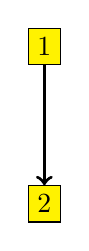
\begin{tikzpicture}
\path (0,4) node[fill=yellow,draw](n1){1}
      (0,2) node[fill=yellow,draw](n2){2};
\draw[->,very thick] (n1.south) -- (n2.north);
% \filldraw[fill=green!20] ellipse (1cm and 4mm);
% \path (-2,2) node[fill=yellow,draw] (eb) {Expected behavior} 
%       (-2,1) node[fill=yellow,draw] (fs) {Formal Specification} 
%       (0,0) node (proof) {Proofs}
%       (2,1) node[fill=blue!30,draw] (pm) {Program Model} 
%       (2,2) node[fill=blue!30,draw] (prog) {Program}; 
% \draw[->,very thick] (eb.south) -- (fs.north);
% \draw[->,very thick,shorten >=5mm] (fs.south) -- (proof.north);
% \draw[->,very thick] (prog.south) -- (pm.north);
% \draw[->,very thick,shorten >=5mm] (pm.south) -- (proof.north);
\end{tikzpicture}
\end{center}

\end{example}

Syntactically, such an advanced loop invariant can be placed anywhere
where an \assert{} clause. The difference is in the
semantics: a loop invariant must be \emph{inductive}. This means that
a proposition given as a loop invariant must not only be true at the
corresponding program point for any execution of the program, but it
must be also preserved indepedently of the context. TODO(citer une ref
a propos des invariants inductifs)

\begin{example}
The program
\begin{c}
  int x = 0;
  int y = 10;

  /*@ loop invariant 0 <= x < 11;
    @*/
  while (y > 0) {
    x++;
    y--;
  }
\end{c}
is not correctly annotated, even if it is true that x remains less
than 11 during the execution. This is because it is not true that the
property $x<11$ is preserved by the execution of \verb|x++ ; y--;|. A
correct loop invariant could be \verb|0 <= x < 11 && x+y == 10|, true
at loop entrance and preserved (under the assumption of the loop
condition \verb|y>0|).

Similarly with general invariants: in
\begin{c}
  int x = 0;
  int y = 10;

  while (y > 0) {
    x++;
    //@ invariant 0 < x < 11;
    y--;
    //@ invariant 0 <= y < 10;
  }
\end{c}
the propositions given as invariants are correct assertions but
not inductive invariants: \verb|0 <= y < 10| is not a consequence of
hypothesis \verb|0 < x < 11| after executing \verb|y--| ; and 
\verb|0 < x < 11| cannot be deduced from \verb|0 <= y < 10| after looping back
through the condition \verb|y>0| and executing \verb|x++|. Correct
invariants could be:
\begin{c}
  while (y > 0) {
    x++;
    //@ invariant 0 < x < 11 && x+y == 11;
    y--;
    //@ invariant 0 <= y < 10 && x+y == 10;
  } 
\end{c}

\end{example}


\subsection{Statement contracts}
\label{sec:statement_contract}


\begin{figure}[t]
  \begin{cadre}
    \begin{syntax}
  statement ::= "/*@" statement-contract "*/" statement
  \
  statement-contract ::= {("for" id ("," id)* ":")?} ;
    simple-behavior-stmt named-behavior-stmt*
  \
  simple-behavior-stmt::=(simple-clauses | abrupt-clause-stmt)*
  \
  named-behavior-stmt ::= "behavior" id ":" behavior-body-stmt
  \
  behavior-body-stmt ::= (assumes-clause |
                     {[not implemented in a named behavior]requires-clause} ;
                    | assigns-clause | ensures-clause ;
                    | abrupt-clauses-stmt) *
\end{syntax}

  \end{cadre}
  \caption{Grammar for statement contracts}
  \label{fig:gram:stcontracts}
\end{figure}


The grammar for statement contracts is given in
Figure~\ref{fig:gram:stcontracts}. It is very similar to function
behaviors, but without \decreases{} clause. Additionally, behavior can
refer to enclosing named behaviors, with the form \texttt{for $id$ :
  \ldots}. Such behaviors are meant to be valid only for the
corresponding function behavior, in particular only under the
corresponding \assumes{} clause.

The clauses \texttt{breaks}, \texttt{continues} and \texttt{returns}
are specific way for stating a property on the program state when the
annotated statement terminates abruptly with the corresponding C
statements, \texttt{break}, \texttt{continue} and \texttt{return}. For the \texttt{returns} case, the \result{} construct is allowed and bound to the value returned (if not a void function).

\begin{example}
  TODO
\end{example}



\oldremark{PC+Claude}{

This allows to pose an assertion on function's state just before it
returns, (whatever way that return occurs) where it is still possible
to refer to local variables.

  avoir la meme chose sur toute fin de bloc.

  Mais il semble que c'est deja prevu... -> A VERIFIER qu'on la bien dit.

  De toute facon, il faut detailler

  Garder l'idee principal: on veut des annotations qui parlent a la
  fois de \result et des variables locales.

  A-t-on besoin de mettre cela pour toute expression ?

  exemple : x = x + (f(..) //@ assert ...\result...) REFUSE'

}




\section{Termination}
\label{sec:termination}

The property of termination concerns both loops and recursive function
calls.
% For that purpose, loops can be annotated with a \texttt{loop
%  variant}\index{loop variant} clause, and functions can be annotated
%with a \decreases{} clause.
Termination is guaranteed by attaching a measure function to each loop
and each recursive functions.

By default, a measure is a function into
integers, and measures are compared using standard less-than ordering
(Section~\ref{sec:integermeasures}). It is also possible to define
measures into other domains and/or using a different ordering relation
(Section~\ref{sec:generalmeasures}).

\subsection{Integer measures}
\label{sec:integermeasures}

Functions are annotated with integer measures with the form
\begin{flushleft}\ttfamily
//@ decreases $e$ ;
\end{flushleft}
and loops are annotated similarly with the form
\begin{flushleft}\ttfamily
//@ loop variant $e$;
\end{flushleft}
where the logic expression $e$ has type \verb|integer|. For recursive calls, or for loops, this expression must decrease for the relation $R$ defined by
\[
R(x,y) ::= x > y ~\verb|&&|~ x \geq 0
\]
In other words, the measure must be a decreasing sequence of integers
which remain non-negative, except possibly for the last value of the
sequence (See example~\ref{ex:loopvariant}).

\begin{example}
  In Example~\ref{ex:bsearch2}, a loop variant \verb|u-l| decreases
  at each iteration, and remains non-negative, except at the last
  iteration where it may become negative.
\end{example}

\subsection{General measures}
\label{sec:generalmeasures}

More general measures on other types can be provided, using the
keyword \verb|for|. For functions it becomes
\begin{flushleft}\ttfamily
//@ decreases $e$ for $R$;
\end{flushleft}
and for loops:
\begin{flushleft}\ttfamily
//@ loop variant $e$ for $R$;
\end{flushleft}
In those cases, the logic expression $e$ has some type $\tau$ and $R$ must be relation on $\tau$, that is a logic binary predicate declared by the form
\begin{flushleft}\ttfamily
//@ predicate $R(\tau~x,\tau~y) \cdots$
\end{flushleft}
(see Section~\ref{sec:logicspec} for details). Of course, to guarantee
termination, it must be proved that $R$ is a well-founded relation.

\begin{example}
  The following is a toy example illustrating a variant annotation
  using a pair of integers, ordered lexicographically.
  \input{lexico.pp}
\end{example}

\subsection{Recursive function calls}

The precise semantics of measures on recursive calls, especially in
the general case of mutually recursive functions, is given as follows.
Each \emph{cluster} of mutually recursive functions must be
identified: each of them corresponds to a strongly connected component of the
call graph.

For a given cluster, each function must be annotated with a decreases
clause with the same relation $R$ (syntactically). Then, in the body
of any function $f$ of that cluster, any recursive call to a function
$g$ must occur in a state where the measure attached to $g$ is smaller
(w.r.t $R$) than the measure of $f$ in the pre-state of $f$. This also
applies when $g$ is $f$ itself.

\begin{example}
  This are the classical factorial and Fibonacci functions
  \input{fact.pp}
\end{example}

\begin{example}
  This example illustrate mutual recursion
  \input{mutualrec.pp}
\end{example}


\section{Logic specifications}
\label{sec:logicspec}

\begin{figure}[t]
  \fbox{\begin{minipage}{0.97\linewidth} \begin{syntax}
  C-external-declaration ::= "/*@" logic-def+ "*/"[These may appear as global \ifCPP{or class} declarations] ;
  \
  logic-def ::= logic-const-def ;
          | logic-function-def ;
          | logic-predicate-def ;
          | lemma-def ;
          | data-invariant-def;
  \
  type-var ::= id
  \
  type-expr ::= type-var ; type variable
  | id;
    "<" type-expr;
    (, type-expr)* ">" ; polymorphic type
  \
  type-var-binders ::= "<" type-var;
                       (, type-var)* ">"
  \
  poly-id ::= ident type-var-binders ; polymorphic object identifier
  \
  logic-const-def ::= "logic" type-expr;
    poly-id "=" term ";"
  \
  logic-function-def ::= "logic" type-expr;
  poly-id parameters "=";
  term ";"
  \
  logic-predicate-def ::=
  "predicate";
  poly-id parameters? "=";
  pred ";"
  \
  parameters ::= "(" parameter;
                 (, parameter)* ")"
  \
  parameter ::= type-expr id
  \
  lemma-def ::= "lemma" poly-id ":";
                   pred ";"
\end{syntax}

    \end{minipage}}
  \caption{Grammar for logic declarations}
\label{fig:gram:logic}
\end{figure}

The language of logic expressions used in annotations can be extended
by declaration of new logic types, and new constants, logic functions
and predicates. These declarations follows the classical setting of
\emph{algebraic specifications}, in particular new functions and
predicates may be either \emph{defined} by explicit expressions, or
\emph{axiomatized} by a set of axioms. The grammer for these declarations is given Figure~\ref{fig:gram:logic}.

\oldremark{Claude}{``logic typedef'' au lieu de ``logic type'' ?
  Non ``type'' et c'est tout
}

The difference between a lemma and an axiom is that a lemma is
supposed to be deductible from axioms: a redundant axioms in some sense.

\subsection{Polymorphic logic types}

\experimental

We consider here an algebraic specification setting based on
multi-sorted logic, where types can be \emph{polymorphic} that is
parameterized by other types. For example, one may declare the type of
polymorphic lists as \input{listdecl.pp} and then can consider for
example list of integers (\texttt{list <integer>}), list of pointers
(e.g. \texttt{list <char*>}), list of list of reals (\texttt{list
  <list <real> >}), etc.

The grammar of Figure~\ref{fig:gram:logic} contains the additional
rules for declaring polymorphic types, and for polymorphic type
expressions.
%Notice that type variables are identifiers preceded by
%the quote character.

\oldremark{All}{
  Plutot que de prefixer les variables de type par dfes backquote, on popurrait mettre des lieurs explicites:

  predicate p<A,B>(A x, B y)

  axiom a<A,B> : ...

}

\subsection{Recursive logic definitions}

The explicit definitions of logic functions and predicates can be
recursive. Declarations in the same bunch of logic declarations are
implicitely mutually recursive, so mutually recursive functions are
possible too.

\begin{example}
  The following logic declaration
  \input{max_index.pp}
  defines a logic function which returns the maximal index $i$ between
  $0$ and $n-1$ such that $t[i]=0$.
\end{example}

%\begin{example} The following introduce $n$-ary trees using list of children.
%  \input{mutualrec.pp}
%\end{example}

Notice that there is no syntactic condition on such recursive
definitions, such as limitation to primitive recursion like e.g. in
Coq~\cite{Coq}. In essence, a recursive definition of the form
$f(args) { e }$ where $f$ occurs in expression $e$ is just a shorcut
for a declaration of $f$ followed by an axiom $\Forall args, f(args) =
e$. In other words, recursive definitions are not guaranteed to be
consistent, ion the same way that axioms may introduce
inconsistency. Of course, tools might provide a way to check
consistency.

\subsection{Higher-order logic constructions}

\experimental

\begin{figure}[t]
  \fbox{\begin{minipage}{0.97\linewidth}
      \begin{syntax}
term ::= "\lambda" binders ";" term ; abstraction
| extended-quantifier "(" term "," term "," term ")"
\
extended-quantifier ::= "\max" | "\min" | "\sum" | "\product"
                      | "\numof"
\end{syntax}
    \end{minipage}}
  \caption{Grammar for higher-order constructs}
\label{fig:gram:higherorder}
\end{figure}

Figure~\ref{fig:gram:higherorder} introduces new term constructs for
higher-order logic.
\begin{description}
\item[Abstraction] The term $\verb|\lambda|~\tau~x_1,\ldots,x_n ~;~ t$
  denotes the $n$-ary logic function which maps $x_1,\ldots,x_n$ to
  $t$. It has the same precedence as \Forall and \Exists
\item[Extended quantifiers] Terms $quant(t_1,t_2,t_3)$ where $quant$
  is \verb|max|, \verb|min|, \verb|sum|, \verb|product|,or
  \verb|num_of|, are extended quantifications. $t_1$ and $t_2$ must
  have type \verb|integer|, and $t_3$ must be a unary function with an
  integer argument, and a numeric value (integer or real) except for
  \verb|\num_of| for which it should have a boolean value. Their
  meanings are given as follows:
  \begin{eqnarray*}
    \verb|\max|(i,j,f) &=& \max \{ f(i),f(i+1), \ldots, f(j) \} \\
    \verb|\min|(i,j,f) &=& \min \{ f(i),f(i+1), \ldots, f(j) \} \\
    \verb|\sum|(i,j,f) &=& f(i)+f(i+1)+\cdots+f(j) \\
    \verb|\product|(i,j,f) &=& f(i)\times f(i+1) \times \cdots \times f(j) \\
    \verb|\num_of|(i,j,f) &=& \# \{ k \mid i \leq k \leq j ~\verb|&&|~ f(k) \} \\
&=& \verb|\sum|(i,j,\verb|\lambda|~\verb|integer|~k ; f(k) ? 1 : 0)
  \end{eqnarray*}
  If $i>j$ then \verb|\sum| and \verb|num_of| above are 0,
  \verb|\product| is 1, and \verb|\max| and \verb|\min| are
  unspecified (see Section~\ref{sec:twovaluedlogic}).
\end{description}


\begin{example}
  Function that sums the element of an array of doubles.
  \input{sum.pp}
\end{example}

\subsection{Concrete logic types}

\begin{figure}[t]
  \fbox{\begin{minipage}{0.97\linewidth}
      \begin{syntax}
  logic-type-decl ::= "type" logic-type = logic-type-def ";"  
  \
  logic-type-def ::= record-type | sum-type ; 
  | type-expr ; type abbreviation 
  \
  record-type ::= "{" type-expr id ( ";" type-expr id)* ";"? "}" 
  \
  sum-type ::= "|"? constructor ( "|" constructor)* 
  \
  constructor ::= id ; constant constructor
  | id "(" type-expr ("," type-expr)* ")" ; non-constant constructor
  \
  type-expr ::= "(" type-expr ("," type-expr)+ ")" ; product type 
  \
  term ::= term "." id ; record field access
  | "\match" term ";" match-cases ; pattern-matching
  | "(" term ("," term)+ ")" ; tuples
  | "\let" "(" id (, id)+ ")" "=" term ";" term ;
  \
  match-cases ::= "|"? match-case ("|" match-case)* 
  \
  match-case ::= pattern ":" term
  \
  pattern ::= term ; see semantic conditions
\end{syntax}
    \end{minipage}}
  \caption{Grammar for concrete logic types and pattern-matching}
\label{fig:gram:logictype}
\end{figure}

\oldremark{SD6+All}{

  faire une analogie avec les types sommes (de Caml, des spec algebriques)

  c'est plutot des types avec constructeurs dans les spec algebriques

}

\experimental

Logic types may not only be declared but also defined concretely, either under thr form of record types, or of sum types. These definitions may be recursive.
With record types, the field access notation $t.id$ can be used, and for sum types, a pattern-matching construction is available. The grammar rules for these additional constructions are given Figure~\ref{fig:gram:logictype}

\oldremark{All}{

TODO: ajouter les types tableaux logiques: tableaux fonctionnels.

sucre syntaxique: t[i] pour select(t,i),  et dans le cas de code ghost, t[i] = e pour t = store(t,i,e)

Example: n-reines.


}

\begin{example}
  The declaration
  \input{listdef.pp}
  introduce a concrete definition of finite lists. The logic definition
  \input{listlengthdef.pp}
  defines the length of a list by recursion and pattern-matching.
\end{example}


\subsection{Hybrid functions and predicates}
\label{sec:logicalstates}

These are functions or predicates which take both C types and logic
types as arguments. Such a predicate can either be defined with the
same syntax as before, or simply declared, but in the latter case the
declaration should usually be augmented with a \reads{} clause, with
the syntax given on Figure~\ref{fig:gram:logicreads} which extend the
one of Figure~\ref{fig:gram:logic}. This feature is useful when a
function or a predicate is not easily definable, but can be more
easily axiomatized.

Both with direct logic definitions or with logic declarations and
axioms, an hybrid function will usually depend on one or more program
points, because it depends upon memory states, via expressions such as:
\begin{itemize}
\item pointer dereferencing: \verb|*p|, \verb|p->f|
\item array accesses: \verb|t[i]|
\item address operator: \verb|&x|
\item built-in predicates depending on memory: \valid
% \item others ?
\end{itemize}
To make such a definition safe, it is mandatory to add after the
declared identifier a set of labels, between curly braces. Expressions
as above must then be enclosed into the \at{} construct to refer to a
given label. Nevertheless, to ease reading such logic expressions, it
is allowed to forgot a label whenever there is only one label in the
context.

\begin{figure}[t]
  \fbox{\begin{minipage}{0.97\linewidth}
      \begin{syntax}
  logic-function-decl ::= "logic" type-expr id parameters ;
                          reads-clause ";"
  \
  logic-predicate-decl ::= "predicate" id parameters ;
                          reads-clause ";"
  \
  reads-clause ::= "reads" locations
  \
  logic-function-def ::= "logic" type-expr id parameters ;
                   reads-clause "{" term "}"
  \
  logic-predicate-def ::= "predicate" id parameters ; 
                          reads-clause "{" pred "}"
  \
  poly-id ::= id ; normal identifier
  | id type-var-binders ; identifier for polymorphic object 
  | id label-binders ; normal identifier with labels
  | id label-binders type-var-binders ; polymorphic identififer with labels
  \ 
  label-binders ::= "{" id (, id)* "}" 
\end{syntax}
    \end{minipage}}
  \caption{Grammar for logic declarations with reads clauses}
\label{fig:gram:logicreads}
\end{figure}


\begin{example}
  The following declares a predicate which tells the number of
  positive elements in an array of doubles, between given indexes
  \input{num_of_pos.pp}
  It should be noticed that without the reads
  clauses, this axiomatization would be inconsistent, since the
  predicate would not depend on the values stored in t, hence the two
  last axioms would say both that $a=b+1$ and $a=b$ for some $a$ and
  $b$.
\end{example}

\begin{example}

  \input{nb_occ.pp}

  \input{permut.pp}

\end{example}

\oldremark{SD7+All}{

As examplified above, hybrid predicates and functions should be used
with caution, since they do not depend only on the values of their
parameters but also in an implicit way on the values stored in memory.


  reutiliser l'exemple en question ? (en le faisant mieux)

}

\subsection{Model variables and model fields}

%\experimental

A model variable is a variable introduced in the specification, whose
type is a logic type. Analogously, structures may have \emph{model
  fields}.  These are used to provide abstract specifications to
functions whose concrete implementation must remain private.

\begin{example}
  Here is an example of a specification of a function which generates
  fresh integers. The contract is given in term of a model variable
  which is intended to represent the set of ``forbidden'' values, e.g. that already have been generated.
  \input{gen_spec_with_model.pp}
  The contract is expressed abstractly, telling that
  \begin{itemize}
  \item the forbidden set of values is modified
  \item the result number is not in the set of forbidden values, thus is ``fresh''
  \item the new set of forbidden contains both the returned value and
    the previously forbidden values.
  \end{itemize}
  An implementation of this function might be as follows, where a
  decision has been made to generate values in increasing order, so
  that it suffices to record the last value generated. This decision
  is made explicit by an invariant.
  \input{gen_code.pp}
\end{example}

Informal semantics of model variables is as follows:
\begin{itemize}
\item Model variables can only appear in specifications. They are not lvalues, thus cannot be assigned directly (unlike ghost variables, see below).
\item Nevertheless a function contract might say that a model variable
  is assigned.
\item When a function contract mentions model variables:
  \begin{itemize}
  \item the precondition is implicitely existentially quantified over
    those variables
  \item the post-conditions are universally quantified over the old
    values of model variables, and existentially quantified over the new values.
  \end{itemize}
\end{itemize}
Thus, in practice the only way of proving that a function body
satisfies a contract with model variables is to provide an invariant
relating model variables and concrete variables, as in the example
above.

\paragraph{Remarks}

Although the syntax of model variables is close to JML model
variables, they differ in the sense that the type of a model variable
is a logic type, not a program type. Also, the semantics above is
closer to the one of the B machines.  It has to be noticed that
program verification with model variables does not have a
well-establish theoretical background~\cite{marche07,leavens07}, so we
deliberately don't provide a precise semantics in this document .


\subsection{Libraries of algebraic specifications}
\label{sec:specmodules}

\experimental

Specification modules can be provided to encapsulate several logic
definitions, for example
\input{listmodule.pp}
Module components are then accessible using a qualified notation like
\verb|List::length|.

Predefined algebraic specifications can be provided as libraries (see
section~\ref{chap:lib}), and imported using a construct like
\input{import.pp} where the file \verb|list.acsl| contains logic
definitions, like the \verb|List| module above.



\section{Pointers and physical adressing}
\label{sec:pointers}

\subsection{Memory blocks and pointer dereferencing}
\label{subsec:memory}

\begin{itemize}
\item \baseaddr{} base address of an allocated pointer
\[
\baseaddr{} : \verb|`a *| \ra \verb|char*|
\]
\item \blocklength{} length of the allocated block of a pointer
\[
\blocklength{} : \verb|`a *| \ra \verb|size_t|
\]

\item $\valid$ is a built-in predicate which applies to a set of terms
  of some pointer type. $\valid(s)$ is true whenever dereferencing any
  $p\in s$ is safe.
\end{itemize}
Some shortcuts are provided:
\begin{itemize}
\item $\verb|\null|$ is an extra notation for the null pointer (i.e. a shortcut for \verb|(void*)0|)
% \footnote{or to \texttt{NULL}, if
%    annotations are pre-processed are the appropriate inclusion of
%    \texttt{stddef.h} is added}
\item $\offset(p)$ returns the offset between p and its base address

  \begin{eqnarray*}
    \offset &:& \verb|`a *| \ra \verb|size_t|  \\
    \offset(p) &=& (\verb|char*|)p - \baseaddr(p)
  \end{eqnarray*}
  the following property holds: for any set of pointers $s$, $\valid(s)$ if and only if for all $p\in s$:
  \[
    \offset(p) \geq 0 \land \offset(p) + \verb|sizeof|(*p) \leq \blocklength(p)
\]

\end{itemize}

\subsection{Separation}

%pointer separation :
%\[
%p \not\equiv q := \baseaddr(p) \neq \baseaddr(q) \lor |(\verb|char*|)p - (\verb|char*|)q| \geq \max(\sizeof(p),\sizeof(q))
%\]

\experimental

$\separated(loc_1,..,loc_n)$ : means that for each $i\neq j$, the intersection of $loc_i$ and $loc_j$ is empty. Each $loc_i$ is a set of terms as defined in
Section~\ref{sec:locations}.

\subsubsection{Locations as first-class values}

Locations, as defined in Section~\ref{sec:locations}, can be used as
first-class values in annotations. They have the built-in type
$loc<A>$ where $A$ is the type of values in that locations.

\begin{example}
  Here is an example where we defined the \emph{footprint} of a
  structure.

  \input{footprint.pp}

  This logic function can be used as argument of \separated.
\end{example}

Note: in other words, a clause assigns l1,..,ln could be transformed
into an post-condition
\[
\forall char* p; \separated(\union(l1,..,ln),*p) ==> *p == \old(*p)
\]



\subsection{Allocation and deallocation}

\experimental

\oldremark{PC}{

quid de la pile -> a voir

}

\begin{itemize}
\item built-in predicate \fresh, specifying in a post-condition that a
  pointer was not allocated in the pre-state.

\item built-in predicate \freed, specifying in a post-condition that a
  pointer was allocated in the pre-state but not anymore.
\end{itemize}

\section{Abnormal termination}

\experimental

It is used to give behavioral properties to the \verb|main| function
or to any function that may exit the program, e.g. calling \verb|exit|
function.

Such a behavior can be written with the form
\begin{verbatim}
  exit_behavior
    assumes
    assigns
    ensures ...
\end{verbatim}
where in ensures clause, \result is bound to the return code, e.g the
value returned by \verb|main| or the argument passed to \verb|exit|.

\oldremark{PC}{

  utilite de la clause assigns ?

  probleme de l'exclusion avec les autres comportements. -> postassumes...

}

\section{Dependencies information}

\experimental

An extended syntax of \assigns clauses allows to give dependencies:
\begin{flushleft}
//@ assigns $loc_1,\ldots,loc_n$ \textbackslash{}from $loc'_1,\ldots,loc'_k$ ;
\end{flushleft}
Moreover, dependencies can be made precise using \emph{functional expressions}:
\begin{flushleft}
//@ assigns $loc$ \textbackslash{}from $loc'_1,\ldots,loc'_k$ = term ;
\end{flushleft}

\experimental

Useful additional constructs for such functional expressions are constructions  of functional arrays :
\begin{itemize}
\item functional update of array : $\{ t[i] \verb|<-| e \} $
\item functional update of struct : $\{ s.f \verb|<-| e \} $
\item arrays or structs given extensionaly, syntax like for C initializers : $\{ t_1, \ldots, t_n \}$
\end{itemize}
%trouver une syntaxe pour introduire les noms des fonctions implicites
%derriere la construction

\oldremark{PC}{

  Ne comprends pas ce que ca veut dire

}

\section{Data invariants}
\label{sec:invariants}


Data invariants are properties on data that are supposed to hold permanently during the life of these data. In ACSL, we distinguish between
\begin{itemize}
\item \emph{global} invariants and \emph{type} invariants: the former
  apply on global variables, whereas the latter are associated to
  static types, and apply on any variables of this type.
\item \emph{strong} invariants and \emph{weak} invariants: strong
  invariants must be valid really at any any time of the program
  execution (more precisely at any \emph{sequence point} as defined in
  the norm TODO: give a reference), whereas weak invariants are valid
  at \emph{function boundaries} (function entrance and exit) but
  cannot be violated in between.
\end{itemize}

\begin{figure}[t]
  \fbox{\begin{minipage}{0.97\linewidth}
      \begin{syntax}
  declaration ::= "/*@" data-inv-decl "*/"
  \
  data-inv-decl ::= data-invariant | type-invariant
  \
  data-invariant ::= inv-strength? "global" "invariant" id ":" pred ";"
  \
  type-invariant ::= inv-strength? "type" "invariant" id "(" C-type-expr id ")" "=" pred ";"
  \
  inv-strength ::= "weak" | "strong"
\end{syntax}
    \end{minipage}}
  \caption{Grammar for declarations of data invariants}
\label{fig:gram:datainvariants}
\end{figure}

The syntax for declaring data invariants is given in
Figure~\ref{fig:gram:datainvariants}. The strength modifier defaults
to \texttt{weak}.


\begin{example}
  In the following example, we declare
  \begin{enumerate}
  \item a weak global invariant \verb|a_is_positive| which specifies that
    the global variable \texttt{a} should remains positive (weakly, so
    this property might be violated temporarily between functions
    calls)
  \item a strong type invariant for type \verb|temperature|
  \item a weak type invariant on structures \verb|S|.
  \end{enumerate}
  \begin{c}
int a;
//@ global invariant a_is_positive: a > 0

typedef int T;
//@ type invariant T_is_positive(T x) { x > 0 } 

struct S {
  int f;
}
//@ type invariant S_f_is_positive(struct S s) { s.f > 0 } 
\end{c}

\end{example}

\oldremark{SD8}{

  montrer un example qui exprime des proprietes d'initialisation de
  variables globales, i.e un tableau contient des valeurs distinctes 2
  a 2.

}

\begin{itemize}
\item Global invariants: invariants on global variables
\item Type invariants: invariants on struct, union, typedef
\item \experimental: \verb|initially|: predicates that should hold after global
  variables initialization
\end{itemize}


\subsection{Semantics}

The distinction between strong and weak invariants is on the sequence
points were the property is supposed to hold. The distinction between
the global invariants and the type invariants is the set of values on
which they are supposed to hold.

\begin{itemize}
\item Weak global invariants are properties which applies to global
  data and hold at any function entrance and function exit.

\item Strong global invariants are properties which applies to global
  data and hold at any step of execution (starting after
  initialisation of these data).

\item A weak type invariant on a type $\tau$ is supposed to hold at
  any function entrance and exit, and applies to any global variable
  or formal parameter which has static type $\tau$. If the result of
  the function is of type $\tau$, the result is also supposed to
  satisfy its invariant at function exit.

\item A strong type invariant on a type $\tau$ is supposed to hold at
  any state of execution, and applies to any global variable, local
  variable, or formal parameter which has static type $\tau$. If the
  result of the function is of type $\tau$, the result is also
  supposed to satisfy its strong invariant at function exit

\end{itemize}



\begin{example}
  example of strong type invariant:
  TODO

  Such kind of strong invariant might be verified using a model with
  abstract data types. (cf caduceus)

\end{example}

\oldremark{PC}{

  remise en cause de la politique d'invariants



Weak invariants do not hold in any state but can be temporarily violated.
Such invariants are allowed under some sound policy~\cite{barnett04jot}.

}

\oldremark{Claude}{

  il faut decider comment sont lies les declarations d'invariants et
  les type associe'.

Example:


typedef struct S {
  int x;
} S;

void reset(S *p) {
  p->x = 0;
}

//@ type invariant I(S *p) { p.x > 0 }

-> reset ne respecte pas cet invariant
}

\begin{example}
  Here is a longer example, the famous Dijkstra's Dutch flag algorithm.
  \input{flag.pp}
\end{example}

\section{Ghost variables and statements}
\label{sec:ghost}

Ghost variables and statements are like C variables and statements,
but visible only in the specifications. They are introduced by the
\verb|ghost| keyword at the beginning of the annotation
(i.e. \verb|/*@ ghost ... */| or \verb|//@ ghost ...| for a one-line
ghost code, as mentionned in section~\ref{sec:gener-about-annot}).
The grammar is given in Figure~\ref{fig:gram:ghost}, in which only the
first form of annotation is used. In this figure, the \textit{C-*}
non-terminals refer to the corresponding grammar rules of the ISO standard,
without any ACSL extension. Any non terminal of the form
\textit{ghost-non-term} for which no definition is given in the figure
represents the corresponding \textit{C-non-term} entry, in which any
\textit{entry} is substituted by \textit{ghost-entry}.

The variations with respect to the C
grammar are the following:
\begin{itemize}
\item Comments must be introduced by \verb|//| and extend until the
  end of the line (the ghost code itself is placed inside a C
  comment. \verb|/* ... */| would thus lead to incorrect C code).
\item It is however possible to write multi-line annotations for ghost
  code. These annotations are enclosed between \verb|/@| and
  \verb|@/|. As in normal annotations, \verb|@|s at the beginning of a
  line and at the end of the comment (before the final \verb|@/|) are
  considered as blank.
\item Logical types, such as \verb|integer| or \verb|real| are
  authorized in ghost code.
\item A non-ghost function can take ghost parameters. If such a ghost
  clause is present in the declarator, then the list of ghost
  parameters must be non-empty and fixed (no vararg ghost). The call
  to the function must then provide the appropriate number of ghost parameters.
\item Any non-ghost \textit{if-statement} which does not have a non-ghost
  \verb|else| clause can be augmented with a ghost one. Similarly, a non-ghost
  \verb|switch| can have a ghost \verb|default:| clause if it does not
  have a non-ghost one (there are however semantical restrictions for valid
  ghost labelled statements in a switch, see next paragraph for details).
\end{itemize}

\oldremark{All}{

  On veut autoriser \texttt{/@ .. @/} dans les commentaires C, on a en a besoin
  pour annoter le code ghost

  preciser aussi que l'on a le droit de mettre des @ en debut
  de ligne (\texttt{\textbackslash{}n space* @}) et juste avant le \texttt{*/} fermant
  (ou alors, considerer le caractere \texttt{@} juste comme un 'space' ?)


}

\oldremark{JCF et CM}{

les ghosts pourrait etre des types logiques.

et quid de prendre l'addresse d'une variable dans les formules logiques ?
autorise' ?

et de toute facon il y a besoin de critere de separation qui assure
que le code ghost ne change pas la semantique du code C. Cas de champ
ghost dans les structures -> change


}

\experimental

\oldremark{Patrick}{on a besoin de ``ghost braces'' pour
      �crire du ``ghost code'', mais �galement de ``logic braces'' afin de cr�er un
      ``logic statement'' auquel on d�sire associer un ``statement
      behavior''. O� en parler~?
    }

\begin{figure}[t]
  \fbox{\begin{minipage}{0.97\linewidth}
      \begin{syntax}

  ghost-type-specifier ::= C-type-specifier ;
  | {logic-type} \
  logic-def ::= "ghost" ghost-declaration \
  direct-declarator ::= C-direct-declarator ;
    | direct-declarator ;
    "(" C-parameter-type-list? ")";
        "/*@" "ghost";
          "(" ghost-parameter-type-list")";
          "*/"; ghost args
        \
  postfix-expression ::= C-postfix-expression ;
    | postfix-expression ;
     "(" C-argument-expression-list? ")";
     "/*@" "ghost" ;
       "(" ghost-argument-expression-list ")";
       "*/" ; call
              ; with ghosts
    \
  statement ::= C-statement ;
             | statements-ghost \
  statements-ghost ::= "/*@" "ghost";
                       ghost-statement+ "*/" \
  ghost-selection-statement ::= C-selection-statement ;
    | "if" "(" C-expression ")";
       statement;
      {"/*@" "ghost" "else"};
      {  ghost-statement+ };
      {  "*/"} \

  struct-declaration ::= C-struct-declaration ;
  | {"/*@" "ghost" };
    { struct-declaration "*/"} ; ghost field

\end{syntax}

%%% Local Variables:
%%% mode: latex
%%% TeX-master: "main"
%%% End:

    \end{minipage}}
  \caption{Grammar for ghost statements}
\label{fig:gram:ghost}
\end{figure}

\oldremark{DD4}{

  Cette grammaire autorise de mettre des ghost dans les ghost, a refaire.

  En fait non, on l'autorise : du code ghost peut avoir besoin
  d'annotation, comme des invariants de boucle

}


\oldremark{All}{

TODO: else ghost

  manque `if () i1 //@ else i2' dans la grammaire

}


\paragraph{Semantics of Ghost Code}

The question of semantics is essential for ghost code. Informally, the
semantics requires that ghost statements do not change the regular
program execution. This implies several conditions, including e.g:
\begin{itemize}
\item Ghost code cannot modify a non-ghost C variable.
\item Ghost code cannot modify a non-ghost structure field.
\item If $p$ is a ghost pointer pointing to a non-ghost memory location, then it is forbidden to assign $*p$.
\item Body of a ghost function is ghost code, hence do not modify
  non-ghost variables or fields.
\item If a non-ghost C function is called in ghost code, it must not
  modify non-ghost variables or fields.
\item If a structure has ghost fields, the \texttt{sizeof} of the
  structure is the same has the structure without ghost fields. Also,
  alignment of fields remains unchanged.
\item The control-flow graph of a function must not be altered by
  ghost statements. In particular, no ghost \verb|return|,
  \verb|goto|, \verb|break|, or \verb|continue| can appear in the body
  of a non-ghost function.
\end{itemize}

Semantics is specified as follows. First, one has to think that
program execution with ghost code involves a \emph{ghost memory heap}
and a \emph{ghost stack}, disjoint from the regular heap and stack.
Ghost variables lie in the ghost heap, so as the ghost field of
structures. Thus, every memory side-effect can be classified as ghost
or non-ghost. Then, the semantics is that memory side-effects of ghost
code must always be in the ghost heap or the ghost stack.

Notice that this semantics is not statically decidable. It is left to
tools to provide approximations, correct in the sense that any code
statically detected as ghost must be semantically ghost.

\begin{example}
  The following example shows some invalid assignments of ghost pointers:
  \input{ghostpointer.pp}
\end{example}

\begin{example}
  The following example shows some invalid ghost statements:
  \input{ghostcfg.pp}
\end{example}

\oldremark{Claude}{
  d'autres exemples, valides ou non valides, serait bienvenus
}

\oldremark{All}{

On veut des tableaux ghost de taille infinie -> cf tableaux fonctionnels de la section sur les assigns from

}

\paragraph{Differences between model variables and ghost variables}


A ghost variable is an additional specification variable which is
assigned in ghost code like any C variable. On the other hand, a model
variable cannot be assigned, but one can state it is modified and can
express properties about the new value, in a non-deterministic way,
using logic assertions and invariants.

In other words, one can say that the specifications stating a ghost
variable modification are executable.

\begin{example}
  \label{ex:gen_code}
  The example~\ref{ex:gen_code} can also be specified with a ghost
  field instead of a model field, by adding before the return :
  \verb|//@ ghost forbidden = union(single(\result),forbidden;|
\end{example}

\subsection{Volatile variables}

TODO

\oldremark{DD1}{

  attacher des fonctions de lecture et d'ecriture a une variable volatile

}

%\section{Module constructions}
%
%\experimental
%
%how to encapsulate several functions...


%\section{Attribute annotations}
%\label{sec:attribute_annot}
%
%\experimental
%
%These are annotations allowing to add attributes on variables, like regular C attributes (const, volatile, restrict).

% The purpose of these are various:
% \begin{itemize}
% \item specific verifications, like \url{http://www.cs.umd.edu/~jfoster/cqual}
% \item specific analyses, like region
%   analyses~\cite{hubert07hav} a la Cyclone~\cite{grossman02pldi}.
% \item allowing to attach model variables/fields to types that are not
%   structures~\cite{filliatr07queens}.
% \end{itemize}

%%% Local Variables:
%%% mode: latex
%%% TeX-PDF-mode: t
%%% TeX-master: "main"
%%% End:
